% Author Vahid Partovi Nia
% Copyright Huawei Technologies
% Network Mind Team



\documentclass[12pt]{beamer}

\usetheme{Hannover}
\setbeamercolor{section in sidebar shaded}{fg=black}

\usecolortheme{beaver}
\beamertemplatenavigationsymbolsempty

%  \usebeamertemplate{navigation symbols}\hfill
%  \insertframenumber{}/\inserttotalframenumber}
  

\useoutertheme{sidebar}
\pgfdeclareimage[width=2.5\baselineskip]{institut-logo}{fig/mcgill_logo}
\setbeamertemplate{footline}
{\raisebox{-2ex}{\pgfuseimage{institut-logo}}
%  \hfill
\hspace{5cm}
  \usebeamertemplate{navigation symbols}
  \insertframenumber{}/\inserttotalframenumber
  \hspace{3.8cm}
YCBS255
}
%\setbeamertemplate{sidebar right}{}
  
\setbeamercolor{block title}{fg=darkred}
\setbeamercolor{local structure}{fg=darkred}

\setbeamercolor{palette sidebar secondary}{fg=darkgray, bg=white}



\usefonttheme{professionalfonts} % using non standard fonts for beamer


\makeatletter
\beamer@nav@subsectionstyle{hide/hide/hide}
\makeatother

\titlegraphic{
\includegraphics[width=2cm]{fig/mcgill_logo}}




\usepackage{listings}
\usepackage{xcolor}
\def \y {\mathbf y}
\def \z {\mathbf z}
\def \Z {\mathbf Z}
\def \X {\mathbf X}
\def \A {\mathbf A}
\def \t {^\top}
\def \inv {^ {-1}}
\def \x {\mathbf x}
\def \bbeta {\boldsymbol \beta}
\def \eeps {\boldsymbol \varepsilon}
\def \TV {\mathrm{TV}}
\def \Radio {\mathrm{Radio}}
\def \Newspaper {\mathrm{Newspaper}}
\def \Sales {\mathrm{Sales}}
\def \Balance {\mathrm{Balance}}
\def \Default {\mathrm{Default}}
\def \M {\mathcal{M}}

\def \r {\mathbf{r}}
\def \e {\mathbf{e}}

\def \RSS {\mathrm{RSS}}

\def \E {\mathrm{E}}
\def \P {\mathbf{P}}

\def \V {\mathrm{V}}
\def \cor {\mathrm{cor}}

\def \SSigma {\boldsymbol{\Sigma}}
\def \LLambda {\boldsymbol{\Lambda}}
\def \pphi {\boldsymbol{\phi}}
\def \PPhi {\boldsymbol{\Phi}}
\def \mmu {\boldsymbol{\mu}}
\def \ttheta {\boldsymbol{\theta}}


\definecolor{capri}{rgb}{0.0, 0.75, 1.0}
\definecolor{darkcyan}{rgb}{0.0, 0.55, 0.55}
\definecolor{deepfuchsia}{rgb}{0.76, 0.33, 0.76}
\begin{document}
% no title and no author on sidebar
\title[]{Trees and Ensemble Methods}   
\author[]{Vahid Partovi Nia} 
\institute{Lecture 08}
\date{}


\makeatletter
  \begin{frame}[plain]
    \hspace*{-\beamer@leftsidebar}%
    \advance\textwidth by \beamer@leftsidebar\relax
    \beamer@leftsidebar=\z@
    \begin{minipage}{\textwidth}\par%
      \maketitle
    \end{minipage}
  \end{frame}
  \makeatother



\frame{\frametitle{Outline}\tableofcontents} 

\setbeamertemplate{sidebar left}[sidebar theme]

\section{CART}
\frame{\frametitle{Classification and Regression Trees}
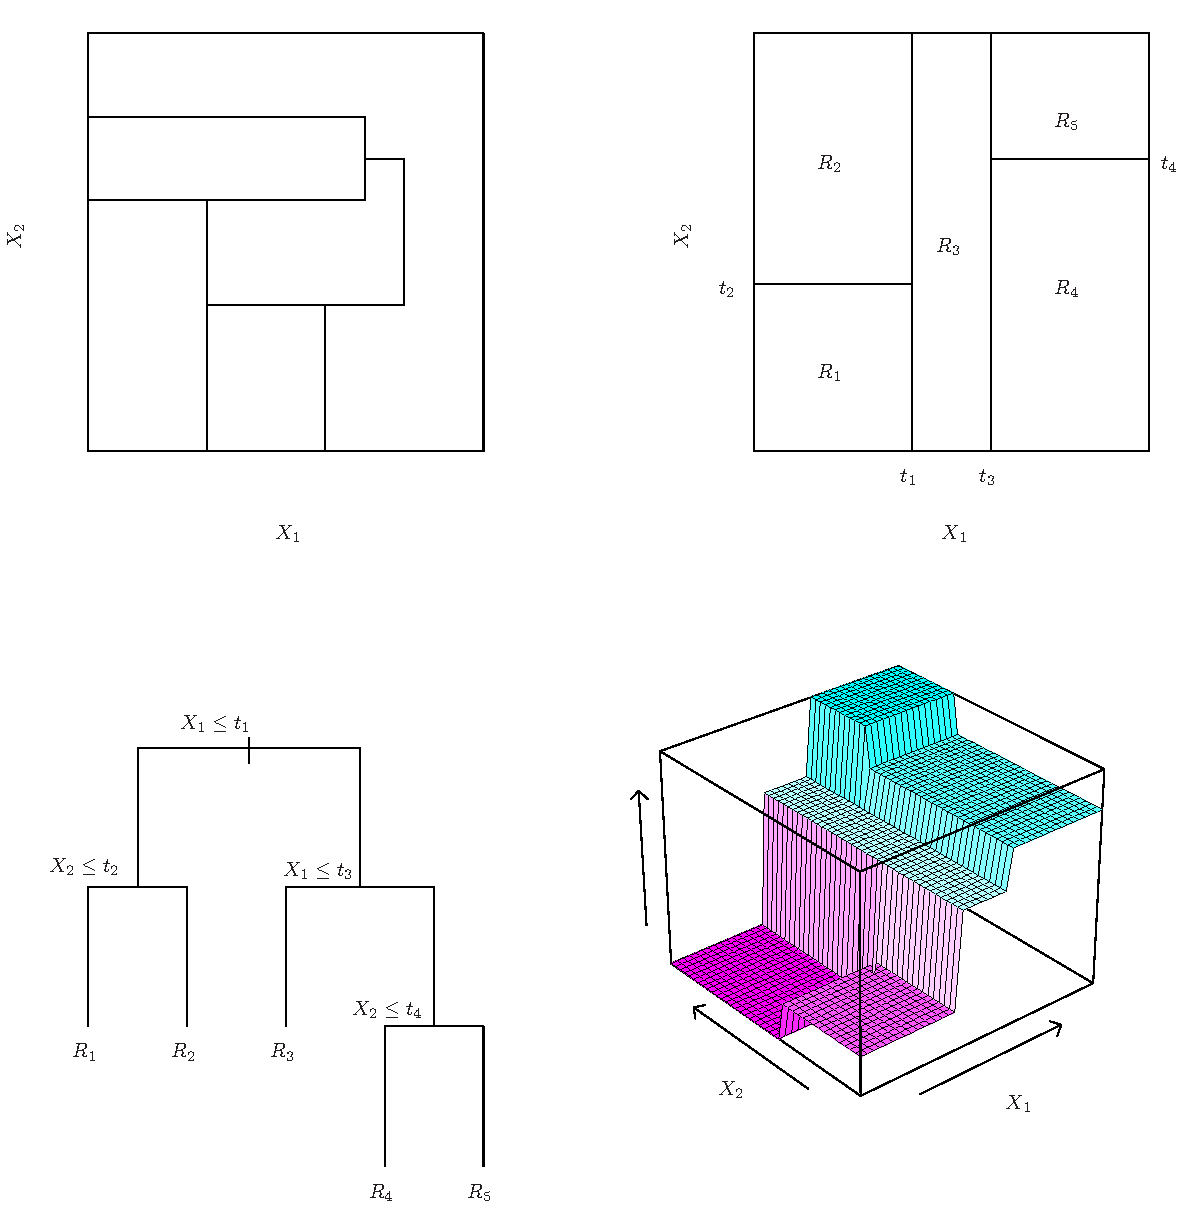
\includegraphics[width=0.8\textwidth]{fig/8-3}
}

\begin{frame}[fragile]\frametitle{}
\tiny	
\begin{lstlisting}
import pandas as pd
path='data/'
filename = path+'spamdata01.csv'
spam = pd.read_csv(filename)
\end{lstlisting} 

\begin{lstlisting}
import matplotlib.pyplot as plt
%matplotlib inline 
plt.scatter(spam.values[:,11], spam.values[:,-1]);
\end{lstlisting} 

\begin{lstlisting}
from sklearn.tree import DecisionTreeClassifier
from sklearn.tree import export_graphviz

dt = DecisionTreeClassifier(max_depth=3)

X = spam.values[:, :57]
y = spam.values[:, -1]
dt.fit(X,y)
spamnames = spam.columns.tolist()[:57]
\end{lstlisting} 

\begin{lstlisting}
dot_data = export_graphviz(dt, out_file=None, 
                         feature_names=spamnames,  
                         class_names=['ham', 'spam'],  
                         filled=True, rounded=True,  
                         special_characters=True)  
\end{lstlisting} 
\begin{lstlisting}
import graphviz
graph = graphviz.Source(dot_data)  
graph 
\end{lstlisting} 
\end{frame}


\frame{\frametitle{}
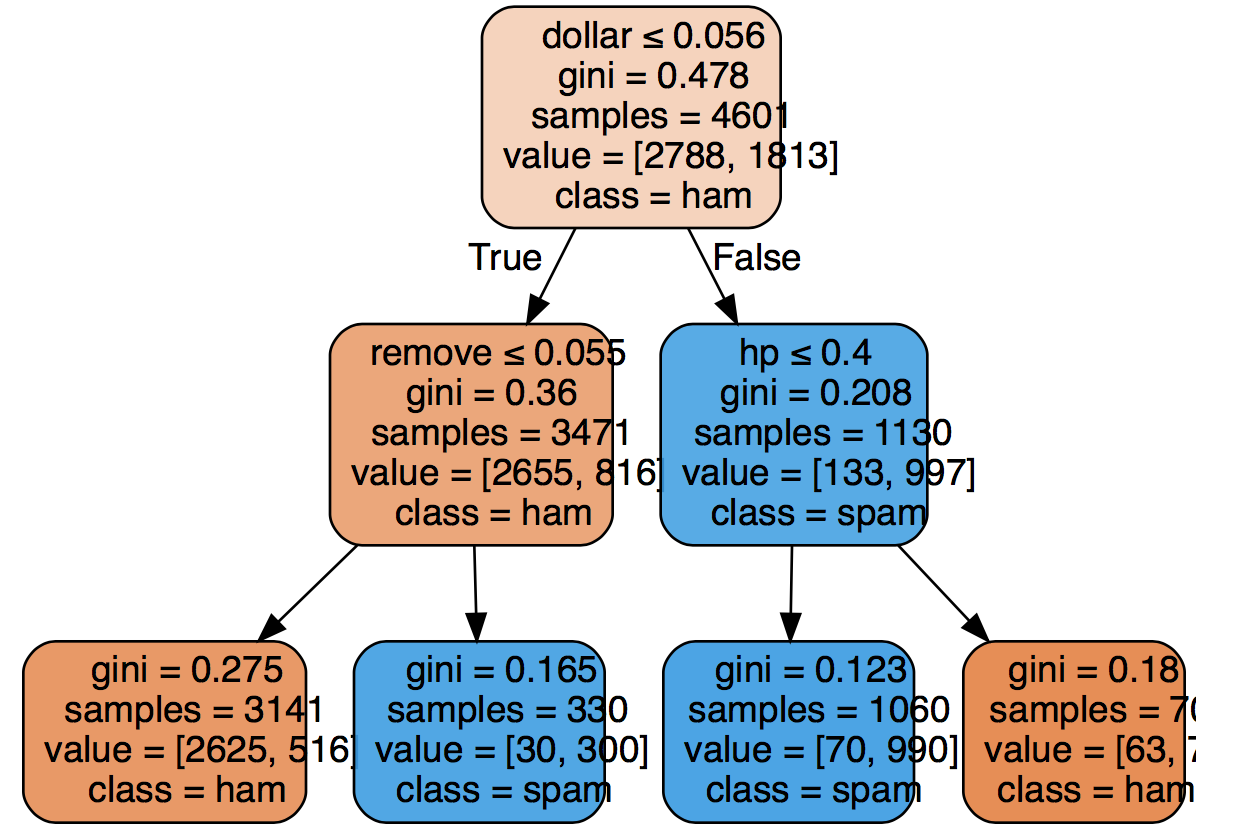
\includegraphics[width=0.9\textwidth]{fig/tree2}
}


\begin{frame}[fragile]\frametitle{}
\tiny	
\begin{lstlisting}
dt10 = DecisionTreeClassifier(max_depth=10)
dt10.fit(X_train,y_train)
y10_pred = dt10.predict(X_test)
\end{lstlisting} 

\begin{lstlisting}
from sklearn.metrics import accuracy_score
accuracy_score(y_test, y10_pred)
\end{lstlisting} 


\begin{lstlisting}

\end{lstlisting} 

\end{frame}
\section{Bagging}
\frame{\frametitle{Bagging}
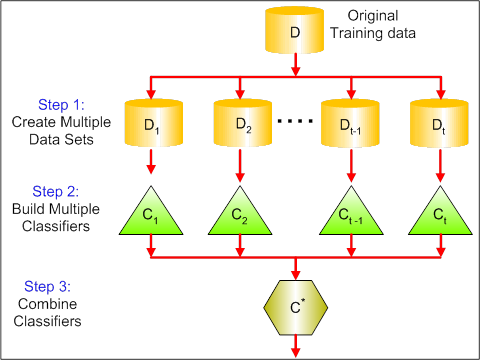
\includegraphics[width=0.8\textwidth]{fig/bagging}
}


\begin{frame}[fragile]\frametitle{}
\tiny	
\begin{lstlisting}
from sklearn.ensemble import BaggingClassifier
bag = BaggingClassifier(n_estimators=100, random_state=1)
bag.fit(X_train, y_train)
y_hat = bag.predict(X_test)
accuracy_score(y_test, y_hat)
\end{lstlisting} 
\end{frame}
\section{Boosting}
\begin{frame}[fragile]\frametitle{}
\tiny	
\url{http://arogozhnikov.github.io/2016/07/05/gradient_boosting_playground.html}
\begin{lstlisting}
from sklearn.ensemble import AdaBoostClassifier
adaboost = AdaBoostClassifier(n_estimators= 100, random_state=1)
adaboost.fit(X_train, y_train)
y_hat = adaboost.predict(X_test)
accuracy_score(y_test, y_hat)
\end{lstlisting} 
\end{frame}




%\frame{\frametitle{}
%\includegraphics[width=0.5\textwidth]{fig/}
%}

%\frame{\frametitle{}
%\includegraphics[width=0.5\textwidth]{fig/}
%}

%\frame{\frametitle{}
%\includegraphics[width=0.5\textwidth]{fig/}
%}
%

%\frame{\frametitle{}
%\includegraphics[width=0.5\textwidth]{fig/}
%}
%
%
%

\end{document}
